\chapter{Nitrogen and Nitrogen Cycle}
Nitrogen is the fourth most abundant element in cellular biomass, and it comprises the majority of Earth’s atmosphere.\cite{stein_nitrogen_2016}. Microbial activity is key in this cycle and 

Wastewater is treated in \gls{asps}. The process of \gls{nitrification} is key.

\subsection{Sample Figure}
You can add figures using the following structure:
\begin{figure}[h!]
    \centering
    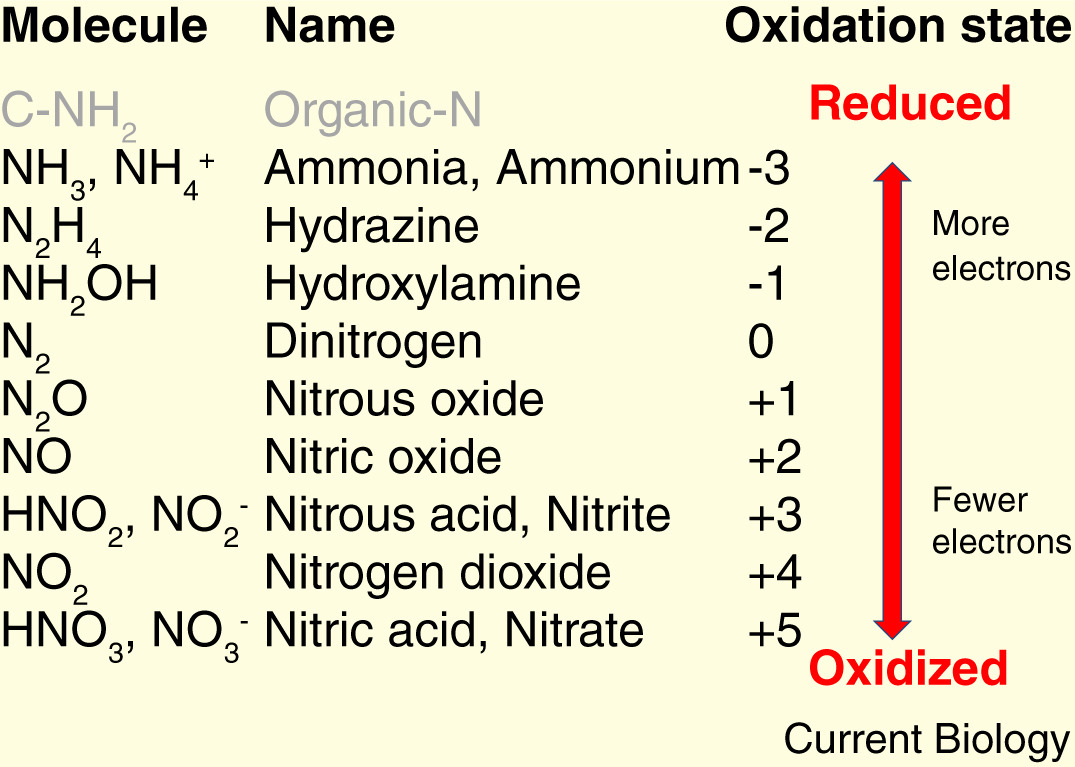
\includegraphics[
        width=0.9\textwidth,
        alt={A diagram showing the nitrogen cycle with different molecules like Ammonia and Nitrite at various oxidation states from -3 to +3.}
        ]
    {images/nitrogen-cycle-intermediates.jpg}
    \caption{Schematic layout of a Waste Stabilization Pond system}
    \label{fig:Nitrogen Cycle}
\end{figure}